\section{Theory and Procedure}
\label{sec:theory}
In this section we describe the procedure and algorithm used to arrive at a function implmentable for the unknown component and also show how we can explore the solution space. We will apply the algorithm on an example to substantiate our theory. 
\subsection{Reference specification is polynomial f}
Consider a specification polynomial $f$ and its circuit implementation $C$, modeled as polynomials $F = \{f_1,\dots,f_s\}\in \mathbb{F}_q[x_1,\dots, x_n]$. The generator of polynomials is given as $J=\langle F \rangle$, with $J_0=\langle x_l^q-x_l\rangle$ being the set of all vanishing polynomials. Let us consider RTTO (\autoref{def:rtto}) as the variable order for the circuit. We will assume $f_i:1\le i \le s$ to be the unknown component which is of the special form:
\begin{gather} 
\label{fiform}
f_i = x_i + P(X_u)
\end{gather}

where $x_i$ is the leading monomial, and $P$ is the tail representing desired solution in variables$:X_u \subset \{x_1,\dots,x_n\} \text{ s.t. } x_j \in X_u \text{ and } x_j<x_i$ in the order. 

As described in ~\autoref{lem:imt} for a correct implementation, specification $f$ should vanish on the variety of ideal generated by the circuit polynomials i.e., $f$ will be in the ideal generated by the circuit:

\begin{equation}
\label{member}
f \in J + J_0; 
f \in \langle f_1,..,f_s\rangle + \langle x_l^q-x_l\rangle;1\le l \le n
\end{equation}
% $f = h_1f_1 + h_2f_2 +\dots+h_if_i+\dots+h_sf_s+H\langle x_i^q-x_i\rangle$
Using Ideal membership testing, we can rewrite $f$ in terms of its generators as:

$f = h_1f_1 + h_2f_2 + \dots+h_if_i+\dots+h_sf_s +H\langle x_l^q-x_l\rangle$

where $H, h_m:1\le m \le s$ are arbitrary elements from $\Fq$.\\
From~\eqref{fiform}:

% $f = h_1f_1 + h_2f_2 +\dots+h_ix_i+h_iP+\dots+h_sf_s+H\langle x_i^q-x_i\rangle$
{\small$f = h_1f_1 + h_2f_2 +\dots+h_ix_i+h_iP(X_u)+\dots+h_sf_s+H\langle x_l^q-x_l\rangle$}

% Given the RTTO $>$, we know the polynomials from $f_s,\dots,f_{i+1}$ and the leading term of $f_i$. Using algorithm:(\ref{algo:mv_reduce}) to reduce 
% $f - h_1f_1 - h_2f_2 -\dots-h_ix_i = h_iP+\dots+h_sf_s+H\langle x_i^q-x_i\rangle$
$f - h_1f_1 -\dots-h_ix_i = h_iP(X_u)+\dots+h_sf_s+H\langle x_l^q-x_l\rangle$

% $f - h_1f_1 - h_2f_2 -\dots-h_ix_i \in \langle h_i,f_{i+1},\dots,f_s, x_i^q-x_i\rangle$
$f - h_1f_1 -\dots-h_ix_i \in \langle h_i,f_{i+1},\dots,f_s, x_l^q-x_l\rangle$\\
We shall call the intermediate remainder computed on the left hand side as $r$.
\begin{equation}
g \in \langle h_i,f_{i+1},\dots,f_s, x_l^q-x_l\rangle
\end{equation}
\begin{figure*}[hbt]
	\begin{center}
	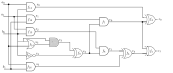
\includegraphics[scale = 0.80]{mas_c}
	\end{center}
	\vspace{-2ex}
	\caption{2-bit Mastrovito multiplier with redundancy}
	\label{mas_c}
	\vspace{-1ex}
\end{figure*}\\
Given polynomials $h_i, g, f_{i+1},\dots,f_s$, we compute $P$ such that:

 $r = Ph_i+h_{i+1}f_{i+1}+\dots+h_sf_s+H\langle x_l^q-x_l\rangle$

The computed $P$ is a solution to the function implemented by the unknown gate. This linear combination computation is done using $lift$ (\autoref{lem:imt}) implementation in SINGULAR~\cite{DGPS_410}.

%add this as a lemma
We will also have cases, when $h_i$ ends up being a constant, in which case $lift$ returns $r$ itself as a solution $h_i^{'}$. To arrive at a implementable solution, we divide $h_i^{'}$ by the constant $h_i$(multiply the inverse of $h_i$) and reduce the result by rest of the input polynomials\{$f_{i-1},\dots,f_1$\}. 

\begin{align}
h_i^{'}h_i^{-1}\xrightarrow[]{f_{i+1}}\xrightarrow[]{f_{i+2}}\dots\xrightarrow[]{f_s}P
\end{align}
Despite being a correct solution, the above approach doesn't guarantee the solution to be in the immediate support variables of $f_i$ due to RTTO$>$. To determine a solution in immediate support variable set $x_j$ of $f_i$, we use an elimination term order (\autoref{def:elim}) for the variables $x_k$ followed by $x_j$. We can then compute a $GB$ using this elimination term order with the intermediate solution $P$ added as tail of $f_i$. This $GB$ will have one and only one polynomial which is of the form $x_k + \mathcal{F}(x_j)$, where $\mathcal{F}$ is the function implemented by the gate, and is the most desired solution. 

Since we found two solutions, it is given that $P$ is not unique. We can explore more such solutions which might satisfy the unknown component functionality. Given $P$ as one of the solutions, under RTTO$>$ we have:

$r = Ph_i+h_{i+1}f_{i+1}+\dots+h_sf_s+H^{'}\langle x_l^q-x_l\rangle;$\\
Since $r$ can be computed as any linear combination of polynomials, we can rewrite the equation as:\\
$Ph_i+h_{i+1}f_{i+1}+\dots+h_sf_s+H^{'}\langle x_l^q-x_l\rangle = P^{1}h_i+h_{i+1}^{'}f_{i+1}+\dots+h_s^{'}f_s+H^{'}\langle x_l^q-x_l\rangle$;\\
Rearranging the terms:

$(P-P^{1})h_i = (h_{i+1}-h_{i+1}^{'})f_{i+1}+\dots+(h_{s}-h_{s}^{'})f_s+(H-H^{'})x_l^q-x_l;$

$(P-P^{1})h_i \in \langle f_{i+1},\dots,f_s,x_l^q-x_l\rangle;$\\
By definition of Quotient of Ideals (\autoref{def:quo}):
\vspace{0.1in}
\begin{equation}
\label{quotcomp}
P-P^{1} \in \langle f_{i+1},\dots,f_s,x_l^q-x_l\rangle:h_i;
\end{equation}

There can be many $P^{*}$'s which might satisfy the above membership test. We can pick any polynomial from the quotient operation, add the previous solution $P$ and compute a new $P$'s. All such $P$'s computed are valid solutions and will satisfy the membership test with specification polynomial $f$. The following example for a redundant boolean logic implementing the majority function demonstrates the above procedure.

\begin{Example}
Consider the 2-bit Mastrovito multiplier with redundancy as shown in~\autoref{mas_c} with variables from ring $\R=\F_2[a_0,b_0,a_1,b_1,s_0,s_1,s_2,s_3,s_4,s_5,e_0,e_1,e_2,e_3,r_0,z_0,$ $z_1,Z,A,B]$.\\%\mathcal{F}(a_1,b_1)$.\\
% For the given circuit, we define \textit{cuts} across the gates based on heuristics such as dependency and levelization\cite{maciej:2016:1}. A $cut$ is defined as a set of signals that separates primary inputs from primary outputs. The prominence of these cuts is to maintain a variable order across cuts . For example at each cut $cut_m$ from the figure(\ref{tianka_ckt_c}), the following variable set has to be maintained across reductions.
% \begin{equation}
% \begin{split}
% cut_0 = \{a,b,c\} &\quad cut_3= \{z_1,z_2\}\\
% cut_1 = \{e_0,e_1,c,e_2\}  &\quad cut_4 = \{z\} \\
% cut_2 = \{e_0,d_0,e_2\}
% \end{split}
% \end{equation}
The 2x2 Mastrovito multiplier with specification $f: Z + A\cdot B$, is constructed as follows:
% \begin{lalign*}
% \begin{split}
\begin{enumerate}
    \item{Field construction: $\F_4 = \F_2[X]$ (mod $\mathcal{P}$); where $\mathcal{P} = X^2 + X + 1$ is the primitive polynomial used.}
    \item{$Z = z_0 +\al z_1; A = a_0 +\al a_1; B = b_0 +\al b_1;$ are the word level polynomials, and $\al$ is the root of primitive polynomial s.t. $\mathcal{P}(\al)=0$.}
\end{enumerate}
Based on the circuit topology, RTTO$>$ with variable order:
$\{Z\}>\{A>B\}>\{z_0>z_1\}>\{r_0\}>\{e_0>e_1\}>\{e_2\}>\{e_3\}>\{s_0>s_1>s_2>s_3>s_4>s_5\}>\{a_0>a_1>b_0>b_1\}$\\ 
Let $F$ be the set of all polynomials implementing the circuit which is given as:
% \begin{equation*}
% \begin{split}
% f_1:s_0 + a_0*b_0;  &  f_5:r_0 + s_1 + s_2; & f_8:A + a_0 + a_1*\al; \\
% f_2:s_3 + \mathcal{F}(a_1,b_1);  &  f_6:z_0 + s_0 + s_3; & f_9:B + b_0 + b_1*\al;\\
% f_3:s_2 + a_1*b_0;  &  f_7:z_1 + r_0 + s_3; & f_{10}:Z + z_0 + z_1*\al;\\
% f_4:s_1 + a_0*b_1;
% \end{split}
% \begin{equation}
{\small\begin{flalign*}
f_1:Z + z_0 +\al z_1;  &\quad f_9:e_2 + e_3 + s_4;   \\
f_2:A + a_0 +\al a_1;  &\quad f_{10}:e_3 + b_0 + s_3; \\
f_3:B + b_0 +\al b_1;  &\quad f_{11}:s_0 + a_0b_0; \\
f_4:z_0 + s_0 + e_0;	&\quad f_{12}:s_1 + a_1b_1; \\
f_5:z_1 + e_0 + r_0;	&\quad f_{13}:s_2 + a_1b_0; \\
f_6:r_0 + e_1 + s_5;	&\quad f_{14}:s_3 + a_0 + b_0 + a_0b_0; \\
f_7:e_0 + s_1e_2;       &\quad f_{15}:s_4 + b_0 + 1;\\
f_8:e_1 + s_2e_2;		&\quad f_{16}:s_5 + a_0b_1;\\
\end{flalign*}}
We shall add the ideal of vanishing polynomials $J_0$ for primary inputs.  
{\small\begin{flalign*}
f_{17}:a_0^2 + a_0; \\
f_{18}:a_1^2 + a_1; \\
f_{19}:b_0^2 + b_0; \\
f_{20}:b_1^2 + b_1; 
\end{flalign*}}%
\begin{small}
$F = \{f_1,\dots,f_{16}\}; J = \langle F\rangle = \langle f_1,\dots,f_{16}\rangle; J_0 = \langle f_{17},\dots,f_{20}\rangle$
\end{small}
% Due to RTTO$>$, the set of polynomials ($J+J_0$) is in itself a \Grobner basis.\\

For a correct implementation, specification $f$ vanishes on circuit implementation~(\autoref{lem:imt}):

% \begin{equation}
$f \in \langle f_1,f_2,f_3,\dots,f_{16}\rangle+\langle f_{17},f_{18}$ $,\dots,f_{20}\rangle$

$f \xrightarrow[]{GB(f_1\dots f_{20})}_0$

% \end{equation}
% h_4f_4 \in \langle f,f_1,f_2,f_3,f_5,f_6,f_7\rangle\\
% h_4f_4 = f+h_1f_1+h_2f_2+h_3f_3+h_5f_5+h_6f_6+h_7f_7
Now, let us assume the marked gate:$f_{10}$ to be the \textit{unknown component} in the design which is of the form $f_{10} = e_3 + P$, where $P$ is the unknown function to be implemented by the gate. We know that under RTTO$>$, the given set of circuit polynomials in itself form a $GB$. Hence to compute $r$, we start reducing the specification polynomial $f$ using polynomials from the set $\langle J + J_0\rangle$. 

We will use the following notations for reduction: '[]' to represent quotient-$h_j$'s, '()' to represent divisor-$f_j$'s, and '\{\}' to represent the partial remainder of every reduction step-$fp_j$'s.

\begin{small}
% \begin{split}
$f\xrightarrow[]{f_{1}}[1](Z + z_0 +\al z_1)+\{ AB+z_0+\al z_1\}\rightarrow fp_1$

$fp_1\xrightarrow[]{f_2}[B](A+a_0+\al a_1)+\{Ba_0+\al Ba_1+z_0+\al z_1\}\rightarrow fp_2$

$fp_2\xrightarrow[]{f_3}[a_0+\al a_1](B+b_0+\al b_1)+\{z_0+\al z_1+\al a_0b_1+a_0b_0+ (\al+1)a_1b_1 + \al a_1b_0\}\rightarrow fp_3$

$fp_3\xrightarrow[]{f_4}[1](z_0+e_0+s_0)+\{\al z_1+e_0+s_0+\al a_0b_1+a_0b_0+(\al+1)a_1b_1+\al a_1b_0\}\rightarrow fp_4$

$fp_4\xrightarrow[]{f_5}[\al](z_1+r_0+e_0)+\{\al z_1+e_0+s_0+\al a_0b_1+a_0b_0+(\al+1)a_1b_1+\al a_1b_0\}\rightarrow fp_5$

$fp_5\xrightarrow[]{f_6}[\al](r_0+e_1+s_5)+\{(\al+1)e_0+\al e_1+s_0+\al s_5+\al a_0b_1+a_0b_0+(\al+1)a_1b_1+\al a_1b_0\}\rightarrow fp_6$

$fp_6\xrightarrow[]{f_7}[\al+1](e_0+e_2*s_1)+\{\al e_1+(\al+1)e_2s_1+s_0+\al s_5+\al a_0b_1+a_0b_0+(\al+1)a_1b_1+\al a_1b_0\}\rightarrow fp_7$

$fp_7\xrightarrow[]{f_8}[\al](e_1+e_2*s_2)+\{(\al+1)e_2s_1+\al e_2s_2 + s_0+\al s_5+\al a_0b_1+a_0b_0+(\al+1)a_1b_1+\al a_1b_0\}\rightarrow fp_8$

$fp_8\xrightarrow[]{f_9}[(\al+1)s_1 + \al s_2](e_2+e_3+s_4)+\{(\al+1)e_3s_1+ \al e_3s_2 +s_0+(\al+1)s_1s_4+\al s_2s_4+\al s_5+\al a_0b_1+a_0b_0+(\al+1)a_1b_1+\al a_1b_0\}\rightarrow fp_9$
\end{small}

\begin{tiny}
% $fp_6\quad\xrightarrow[]{lt(f_2)}[s_3](\underbrace{x+1}_\text{$h_2$})+\{\underbrace{(x)*s_1+(x)*s_2+(x)*a_0*b_1+(x)*a_1*b_0+(x+1)*a_1*b_1}_\text{$r$}\}$
${\scriptstyle fp_9}\xrightarrow[]{{\scriptstyle lt(f_{10})}}[\underbrace{{\scriptstyle (\al+1)s_1+\al s_2}}_\text{$h_{10}$}]({\scriptstyle e_3})+$ 

$\{\underbrace{{\scriptstyle s_0+(\al+1)s_1s_4+\al s_2s_4+\al s_5+\al a_0b_1+a_0b_0+(\al+1)a_1b_1+\al a_1b_0\}}}_\text{$r$}$ 
\end{tiny}
% \end{split}

Reduction order for $f:$

$f\xrightarrow[]{f_{1}}\xrightarrow[]{f_2}\xrightarrow[]{f_3}\xrightarrow[]{f_4}\xrightarrow[]{f_5}\xrightarrow[]{f_6}\xrightarrow[]{f_7}\xrightarrow[]{f_8}\xrightarrow[]{f_9}\xrightarrow[]{lt(f_{10})}r$

% \begin{equation}
% \begin{split}
% h_4f_4+h_1f_1+h_2f_2+h_3f_3 = f+h_5f_5+h_6f_6+h_7f_7;\\
% h_4(d_0+P(e_1,c))+h_1f_1+h_2f_2+h_3f_3 = f+h_5f_5+h_6f_6+h_7f_7;\\
% h_4*d_0+h_4*P(e_1,c)+h_1f_1+h_2f_2+h_3f_3 = f+h_5f_5+h_6f_6+h_7f_7;\\
% h_4*P(e_1,c)+h_1f_1+h_2f_2+h_3f_3 = h_4*d_0+f+h_5f_5+h_6f_6+h_7f_7;\\
% h_4*P(e_1,c)+h_1f_1+h_2f_2+h_3f_3 = e_0*e_2+a*c+a+b*c+b+c;\\
% h_4*P(e_1,c)+h_1f_1+h_2f_2+h_3f_3 = e_0*e_2+a*c+a+b*c+b+c;
% \end{split}
% \end{equation}
Given: $r,h_{10},f_{11},f_{12},f_{13},f_{14},f_{15},f_{16},J_0$, the problem can be formulated as an ideal membership test using~\eqref{member} such that:
\begin{center}
$r \in \langle h_{10},f_{11},f_{12},f_{13},f_{14},f_{15},f_{16}\rangle + \langle J_0\rangle$
\end{center}

The above ideal membership can be computed by expressing $r$ as a linear combination of the member ideal(~\autoref{lem:imt}).
\begin{tiny}
$r = Ph_{10} + h_{11}f_{11} + h_{12}f_{12}+h_{13}f_{13}+h_{14}f_{14}+h_{15}f_{15}+h_{16}f_{16}+HJ_0$ 
\end{tiny}
% Given polynomial $r$ and ideal $J$ in row matrix form($[J+J_0]$) as inputs, and returns a column matrix $[U]$ as output such that:
% \begin{small}
% $f = [U]\cdot [J+J_0]$
% \end{small}

% \begin{equation}
% \begin{split}
% \begin{small}
% $r = \begin{bmatrix} h_2^{'} & h_3^{'} & \dots & H \end{bmatrix} \cdot 
%     \begin{bmatrix} h_2 \\ f_3 \\ \vdots \\ x_n^2 + x_n \end{bmatrix}$
% \end{small}

In our example, polynomial $r$ can be expressed as a linear combination~(\autoref{lem:imt}) in given member ideal as follows: 

% \end{split}
% \end{equation}
\begin{small}
$r = [b_0]h_{10}+[1]f_{11}+[\al+1]f_{12}+[\al s_4 +\al b_0]f_{13}+[0]f_{14}+[(\al+1)s_1+\al a_1b_0]f_{15}+[\al]f_{16}+[0]f_{17}+[0]f_{18}+[0]f_{19}+[0]f_{20}$;
\end{small}

This computed $P=b_0$ is a solution to the \textit{unknown component} $f_{10}$. Given a solution $P$, we can explore the solution space for the gate $f_i$ in terms of variables $x_j$ such that $x_i>x_j$ in the variable order. This can be achieved by computing a quotient of ideals~(\autoref{def:quo}) and using different elimination ideals~(\autoref{def:elimideal}) with desired variables $x_j$ moved to the end of the variable order.

In our example $r$ can be written as any linear combination of the ideals.\\
\begin{tiny}
$r = Ph_{10} + h_{11}f_{11} + h_{12}f_{12}+h_{13}f_{13}+h_{14}f_{14}+h_{15}f_{15}+h_{16}f_{16}+HJ_0$\\ 
$r = P^`h_{10} + h_{11}^`f_{11} + h_{12}^`f_{12}+h_{13}^`f_{13}+h_{14}^`f_{14}+h_{15}^`f_{15}+h_{16}^`f_{16}+H^`J_0$ 
\end{tiny}

Re-writing the above two equations:\\
\begin{tiny}
$(P-P^`)h_{10} = (h_{11}-h_{11}^`)f_{11} + (h_{12}-h_{12}^`)f_{12}+\dots+(h_{16}-h_{16}^`)f_{16}+(H-H^`)J_0$\\
$(P-P^`)h_{10} \in \langle f_{11},f_{12},\dots,f_{16},J_0\rangle$\\
$(P-P^`)\in \langle f_{11},f_{12},\dots,f_{16},J_0\rangle:h_{10}$\\
$(P-P^`)\in Q$
\end{tiny}

The above expression for $Q$ represents the quotient of ideals operation~(\autoref{def:quo}). We can pick any polynomial within desired variable subset $x_j$ from the result of $Q$ and add it to the computed solution $P$ to arrive at a new solution.

Under the current $RTTO>$ variable order, the quotient of ideals operation results in the following polynomials:\\
\begin{small}
$q[1]=b_1b_0+b_1+b_0+1\\
q[2]=(\al+1)b_1+(\al+1)*b_1*b_0+(\al+1)*b_0+(\al+1)\\
q[3]=a_1+1\\
q[4]=s_5+a_0b_1\\
q[5]=s_4+b_0+1\\
q[6]=s_3+a_0b_0+a_0+b_0\\
q[7]=s_2+b_0\\
q[8]=s_1+b_1\\
q[9]=s_0+a_0b_0$
\end{small}

Any $P+q[k]$, where:$1<k<9$, will work as a solution for the \textit{unknown component} $f_{10}$.

Since we know the immediate input variables of the polynomial $f_{10}$ ($b_0,s_3$), we can compute a solution in terms of these variables by using the elimination ideal~(\autoref{def:elimideal}) $Q \cap \Fq[b_0,s_3]$. The quotient operation with the elimination ideal results in:\\
\begin{small}
$q[1]=s_3b_0 + b_0$
\end{small}

Since, there is only one $q$ from the operation, $P+q[1]=s_3b_0$ will work as a solution for the \textit{unknown component}.

\end{Example}

\subsection{Circuit implementation as reference}
Consider a circuit implementation $C$, modeled as polynomials $F = \{f_1,\dots,f_s\}\in \mathbb{F}_q[in_j,x_1,\dots, x_n]$, with $J_1=\langle F \rangle$, $in_j$ as the set of all primary inputs, and $x_n$ as the word level output. Let us assume $f_i:1\le i \le s$ to be the unknown component which is of the special form:
\begin{gather*} 
f_i = x_k + P
\end{gather*}

Let us consider a different circuit $C_1$ as the golden specification which implements the same function as $C$. The reference circuit is modeled as polynomials $Q = \{q_1,\dots q_r\}\in \mathbb{F}_q[in_j,y_1,\dots, y_m]$, with $J_2=\langle Q \rangle$, $in_j$ as the set of all primary inputs, and $y_m$ as the word level output.

To formulate the problem, we will derive a new circuit structure using the above two implementations ($C,C_1$). Primary input set $in_j$ will be used as the common set of inputs for both the circuits, and the word level outputs ($x_n,y_m$) will be mitered using an XOR gate. A new specification polynomial $f$ is derived using the above setup as:
\begin{gather}
f : t(x_n-y_m)
\end{gather}

where, $t$ is the final output of miter gate.

Now, for a correct implementation, specification $f$ should vanish on the variety of ideal generated by the circuit polynomials i.e., $f$ will be in the ideal generated by the circuit:

$f \in J_1 + J_2 + J_0$: where $J_0$ is the set of all vanishing polynomials from circuits $C$, $C_1$ and miter output $t$.

{\small $f \in \langle f_1,\dots,f_s\rangle + \langle q_1,\dots,q_r\rangle + \langle x_l^q-x_l\rangle + \langle y_u^q-y_u\rangle + \langle t^q-t\rangle$; $1\le l \le n,1\le u \le m$}

The problem formulation is now exactly same as~\eqref{member} with $f_i$ from circuit $C$ as the unknown gate. Now, we will follow the same procedure as in the first notion to realize the function of the unknown component. Once a solution has been computed, we can verify the circuit using principles from weak $\it{Nullstellensatz}$ by checking if $GB(J_1+J_2+J_0)=\{1\}$.

% \begin{algorithm}
% \caption{Resolve the unknown component for a given circuit}
% \label{algo:unknownComponent}
% \begin{algorithmic}[1]

% \Procedure{$multi\_variate\_division$}{$F,f$}

% \Procedure{$forward\_lifting$}{}

% \EndProcedure
% \end{algorithmic}
% \end{algorithm}

% Thus, $P(u_1)=P(e_1,c)=c$, which can implemented as a simple AND gate with $c$ as both inputs. 

% \begin{figure}[ht]
% 	\begin{center}
% 	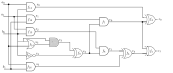
\includegraphics[scale = 0.40]{mas_c}
% 	\end{center}
% 	\vspace{-1ex}
% 	\caption{correct implementation mastrovito}
% 	\label{mas_c}
% 	\vspace{-1ex}
% \end{figure}

% \begin{figure}[ht]
% 	\begin{center}
% 	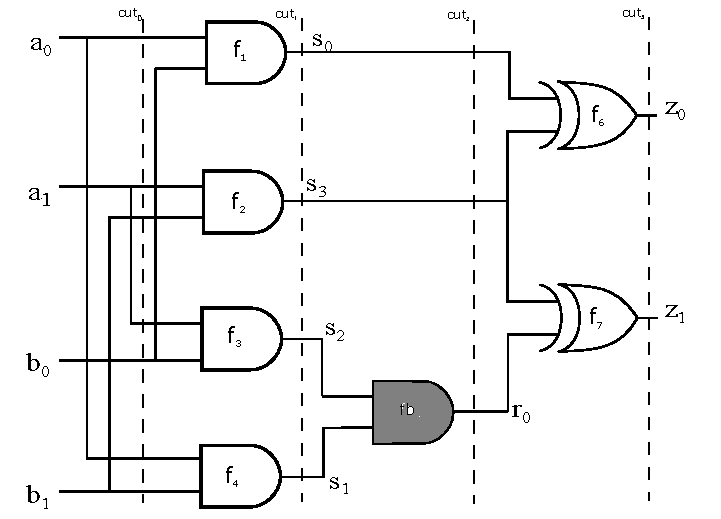
\includegraphics[scale = 0.40]{mas_b}
% 	\end{center}
% 	\vspace{-4ex}
% 	\caption{buggy implementation mastrovito}
% 	\label{mas_b}
% 	\vspace{-2ex}
% \end{figure}